\section{Технологическая часть}

В данном разделе проведен выбор инструментов разработки (языка программирования, библиотек и фреймворков). 
Также приведено обоснование выбора Postgres в качестве СУБД. 
Помимо этого, представлены детали реализации приложения и продемонстрирован интерфейс для взаимодействия с приложением.

\subsection{Выбор СУБД}

В аналитическом разделе при выборе типа модели баз данных была выбрана реляционная модель, следовательно выбор СУБД будет производиться для реляционной модели баз данных. Рассмотрим только самые популярные из них: MySQL, Oracle, PostgreSQL \cite{postgres}, Microsoft SQL Server и SQLite.

Выделим следующие критерии для сравнения выбранных СУБД:

\begin{enumerate}
	\item открытый исходный код;
	\item возможность создания пользователей на уровне БД;
	\item опыт работы с СУБД (не является основным требованием, но желательным).
\end{enumerate}

Результаты сравнения выбранных СУБД по заданным критериям представлены в таблице \ref{tbl:compare_DBMS}.


\begin{table}[ht!]
	\centering
	\caption{Сравнение выбранных СУБД}
	\label{tbl:compare_DBMS}
	\begin{tabular}{|l|l|l|l|l|l|}
		\hline
		\textbf{Критерий} & \textbf{MySQL} & \textbf{Oracle} & \textbf{PostgreSQL} & \textbf{Microsoft SQL Server} & \textbf{SQLite} \\ \hline
		
		1 & + & - & + & - & + \\ \hline
		2 & + & + & + & + & - \\ \hline
		3 & - & - & + & - & + \\ \hline
		
	\end{tabular}
\end{table}

Помимо указанных выше особенностей, стоит отметить, что PostgreSQL активно поддерживается сообществом. На момент 20.05.2023 последнее изменение в исходный код было внесено менее 24 часов назад \cite{postgres-github}.

По результатам сравнения в качестве СУБД для реляционной базы данных был выбран PostgreSQL.

\subsection{Выбор поисковой базы данных}

Постановка задачи предполагает возможность осуществления быстрого поиска событий (с использованием фильтрации, сортировки и пагинации). Такой функционал предоставляет поисковая база данных ElasticSearch \cite{elastic}. Выбор именно этой поисковой БД обоснован возможностью настраивать поиск событий с использованием различных видов фильтрации (включая нечеткое сопоставление), а также поддержкой сортировки событий согласно набранному ими при фильтрации баллу (\textit{\_score}). 

\subsection{Выбор средств реализации}

В качестве используемого языка программирования был выбран Golang. Для реализации приложения на этом языке использовались следующие библиотеки:
\begin{itemize}[]
	\item .ent \cite{ent} --- ORM для взаимодействия с базой данных;
	\item pq \cite{pq} --- драйвер для работы с PostgreSQL;
	\item gqlgen \cite{gqlgen} --- библиотека для реализации GraphQL API.
	\item fx \cite{fx} --- система для управления зависимостями.
\end{itemize}

В качестве среды разработки использовалась среда GoLand.

\subsection{Реализация приложения}

В данном подразделе приведены листинги кода реализуемого приложения.

\subsubsection{Описание таблиц базы данных}

На листингах \ref{lst:events} - \ref{lst:users} приведен код описания таблиц \textit{events} и \textit{users} соответственно.

\begin{center}
\captionsetup{justification=raggedright,singlelinecheck=off}
\begin{lstlisting}[label=lst:events,caption=Описание таблицы событий]
// Fields of the Event.
func (Event) Fields() []ent.Field {
	return []ent.Field{
		field.Time("timestamp"),
		field.String("name"),
		field.String("description").Optional().Nillable(),
		field.String("type"),
		field.Bool("is_whole_day"),
		field.String("creator_uuid").SchemaType(map[string]string{
			dialect.Postgres: "uuid",
		}),
	}
}

// Edges of the Event.
func (Event) Edges() []ent.Edge {
	return []ent.Edge{
		edge.To("tags", Tag.Type).StorageKey(
		edge.Table("events_tags"), edge.Columns("event_uuid", "tag_uuid"),
		),
		edge.To("invitations", Invitation.Type),
		edge.From("creator", User.Type).
		Ref("created_events").
		Field("creator_uuid").
		Unique().
		Required(),
	}
}
\end{lstlisting}
\end{center}

\clearpage

\begin{center}
	\captionsetup{justification=raggedright,singlelinecheck=off}
	\begin{lstlisting}[label=lst:users,caption=Описание таблицы пользователей]
// Fields of the User.
func (User) Fields() []ent.Field {
	return []ent.Field{
		field.String("phone").Unique(),
		field.String("login").Unique(),
		field.String("password_hash"),
		field.String("role").GoType(roles.Type("")),
	}
}

// Edges of the User.
func (User) Edges() []ent.Edge {
	return []ent.Edge{
		edge.To("invitations", Invitation.Type),
		edge.To("created_events", Event.Type),
	}
}
	\end{lstlisting}
\end{center}

\subsubsection{Создание процедуры}

В предыдущем разделе была спроектирована хранимая процедура \linebreak \textit{before\_each\_query}. Реализация этой процедуры с использованием языка plpgsql приведена на листинге \ref{lst:func}.

\begin{center}
	\captionsetup{justification=raggedright,singlelinecheck=off}
	\begin{lstlisting}[label=lst:func,caption=Реализация процедуры before\_each\_query]
CREATE OR REPLACE PROCEDURE before_each_query(IN user_uuid uuid)
	LANGUAGE plpgsql
AS
$$
DECLARE
	role_name regrole;
BEGIN
	role_name = (SELECT role FROM users WHERE users.uuid = user_uuid)::regrole;
	execute format('SET role %I', role_name);
	execute format('SET app.user_uuid = %L', user_uuid);
END;
$$;
	\end{lstlisting}
\end{center}

\subsubsection{Создание ролей и выделение им прав}

В аналитическом разделе была разработана ролевая модель, включающая следующие роли:
\begin{itemize}
	\item simple\_user --- обычный пользователь;
	\item premium\_user --- привелегированный пользователь;
	\item admin --- администратор системы.
\end{itemize}

В соответствии с разработанной диаграммой вариантов использования (рисунки \ref{fig:use-case-simple} -- \ref{fig:use-case-admin}) пользователя были выделены права. Помимо этого, были созданы политики для ограничения доступа на уровне строк (RLS) к таблице пользователей. Создание ролей, выделение им прав и создание политик представлено на листинге \ref{lst:roles}.

\begin{center}
	\captionsetup{justification=raggedright,singlelinecheck=off}
	\begin{lstlisting}[label=lst:roles,caption=Описание ролей]
create role admin;
create role simple_user;
create role premium_user;

grant all on all tables in schema public to admin;

grant select, update (login, phone, password_hash) on users to simple_user;
grant select on access_rights to simple_user;
grant all on events to simple_user;
grant all on invitations to simple_user;
grant all on events_tags to simple_user;
grant select on tags to simple_user;

grant select, update (login, phone, password_hash) on users to premium_user;
grant select on access_rights to premium_user;
grant all on events to premium_user;
grant all on invitations to premium_user;
grant all on events_tags to premium_user;
grant all on tags to premium_user;

ALTER TABLE users
	ENABLE ROW LEVEL SECURITY;

DROP VIEW IF EXISTS session;
CREATE VIEW session AS
SELECT current_setting('app.user_uuid')::uuid AS user_uuid;

grant all on session to simple_user, premium_user, admin;

DROP POLICY IF EXISTS users_select ON users;
CREATE POLICY users_select
	ON users
	FOR SELECT
	USING (true);

DROP POLICY IF EXISTS users_update ON users;
CREATE POLICY users_update
	ON users
	FOR UPDATE
	TO simple_user, premium_user
	USING (uuid = (select user_uuid from session));

DROP POLICY IF EXISTS users_update_admin ON users;
CREATE POLICY users_update_admin
	ON users
	FOR UPDATE
	TO admin
	USING (true);

DROP POLICY IF EXISTS users_delete_admin ON users;
CREATE POLICY users_delete_admin
	ON users
	FOR DELETE
	TO admin
	USING (true);
\end{lstlisting}
\end{center}
\clearpage

\subsubsection{Интерфейс приложения}

Для взаимодействия с приложением был разработан API, обрабатывающий запросы согласно спецификации GraphQL. Для пользователей, событий и тегов были реализованы запросы для получения (всех или по идентификатору), создания, обновления и удаления этих сущностей. Для прав доступа к событиям были реализованы запросы только для их получения. Также был реализован запрос для принудительной синхронизации состояния ElasticSearch с текущим состоянием Postgres. Помимо этого, были реализованы запросы для генерации тестовых данных пользователей, тегов и событий с приглашениями.

Для удобной и быстрой отправки запросов приложение предоставляет специализированный пользовательский интерфейс Apollo Sandbox \cite{sandbox}. На рисунках \ref{fig:search-events} -- \ref{fig:login} приведены несколько примеров запросов к приложению и ответы приложения на эти запросы с использованием этого интерфейса.

\begin{figure}[ht!]
	\centering
	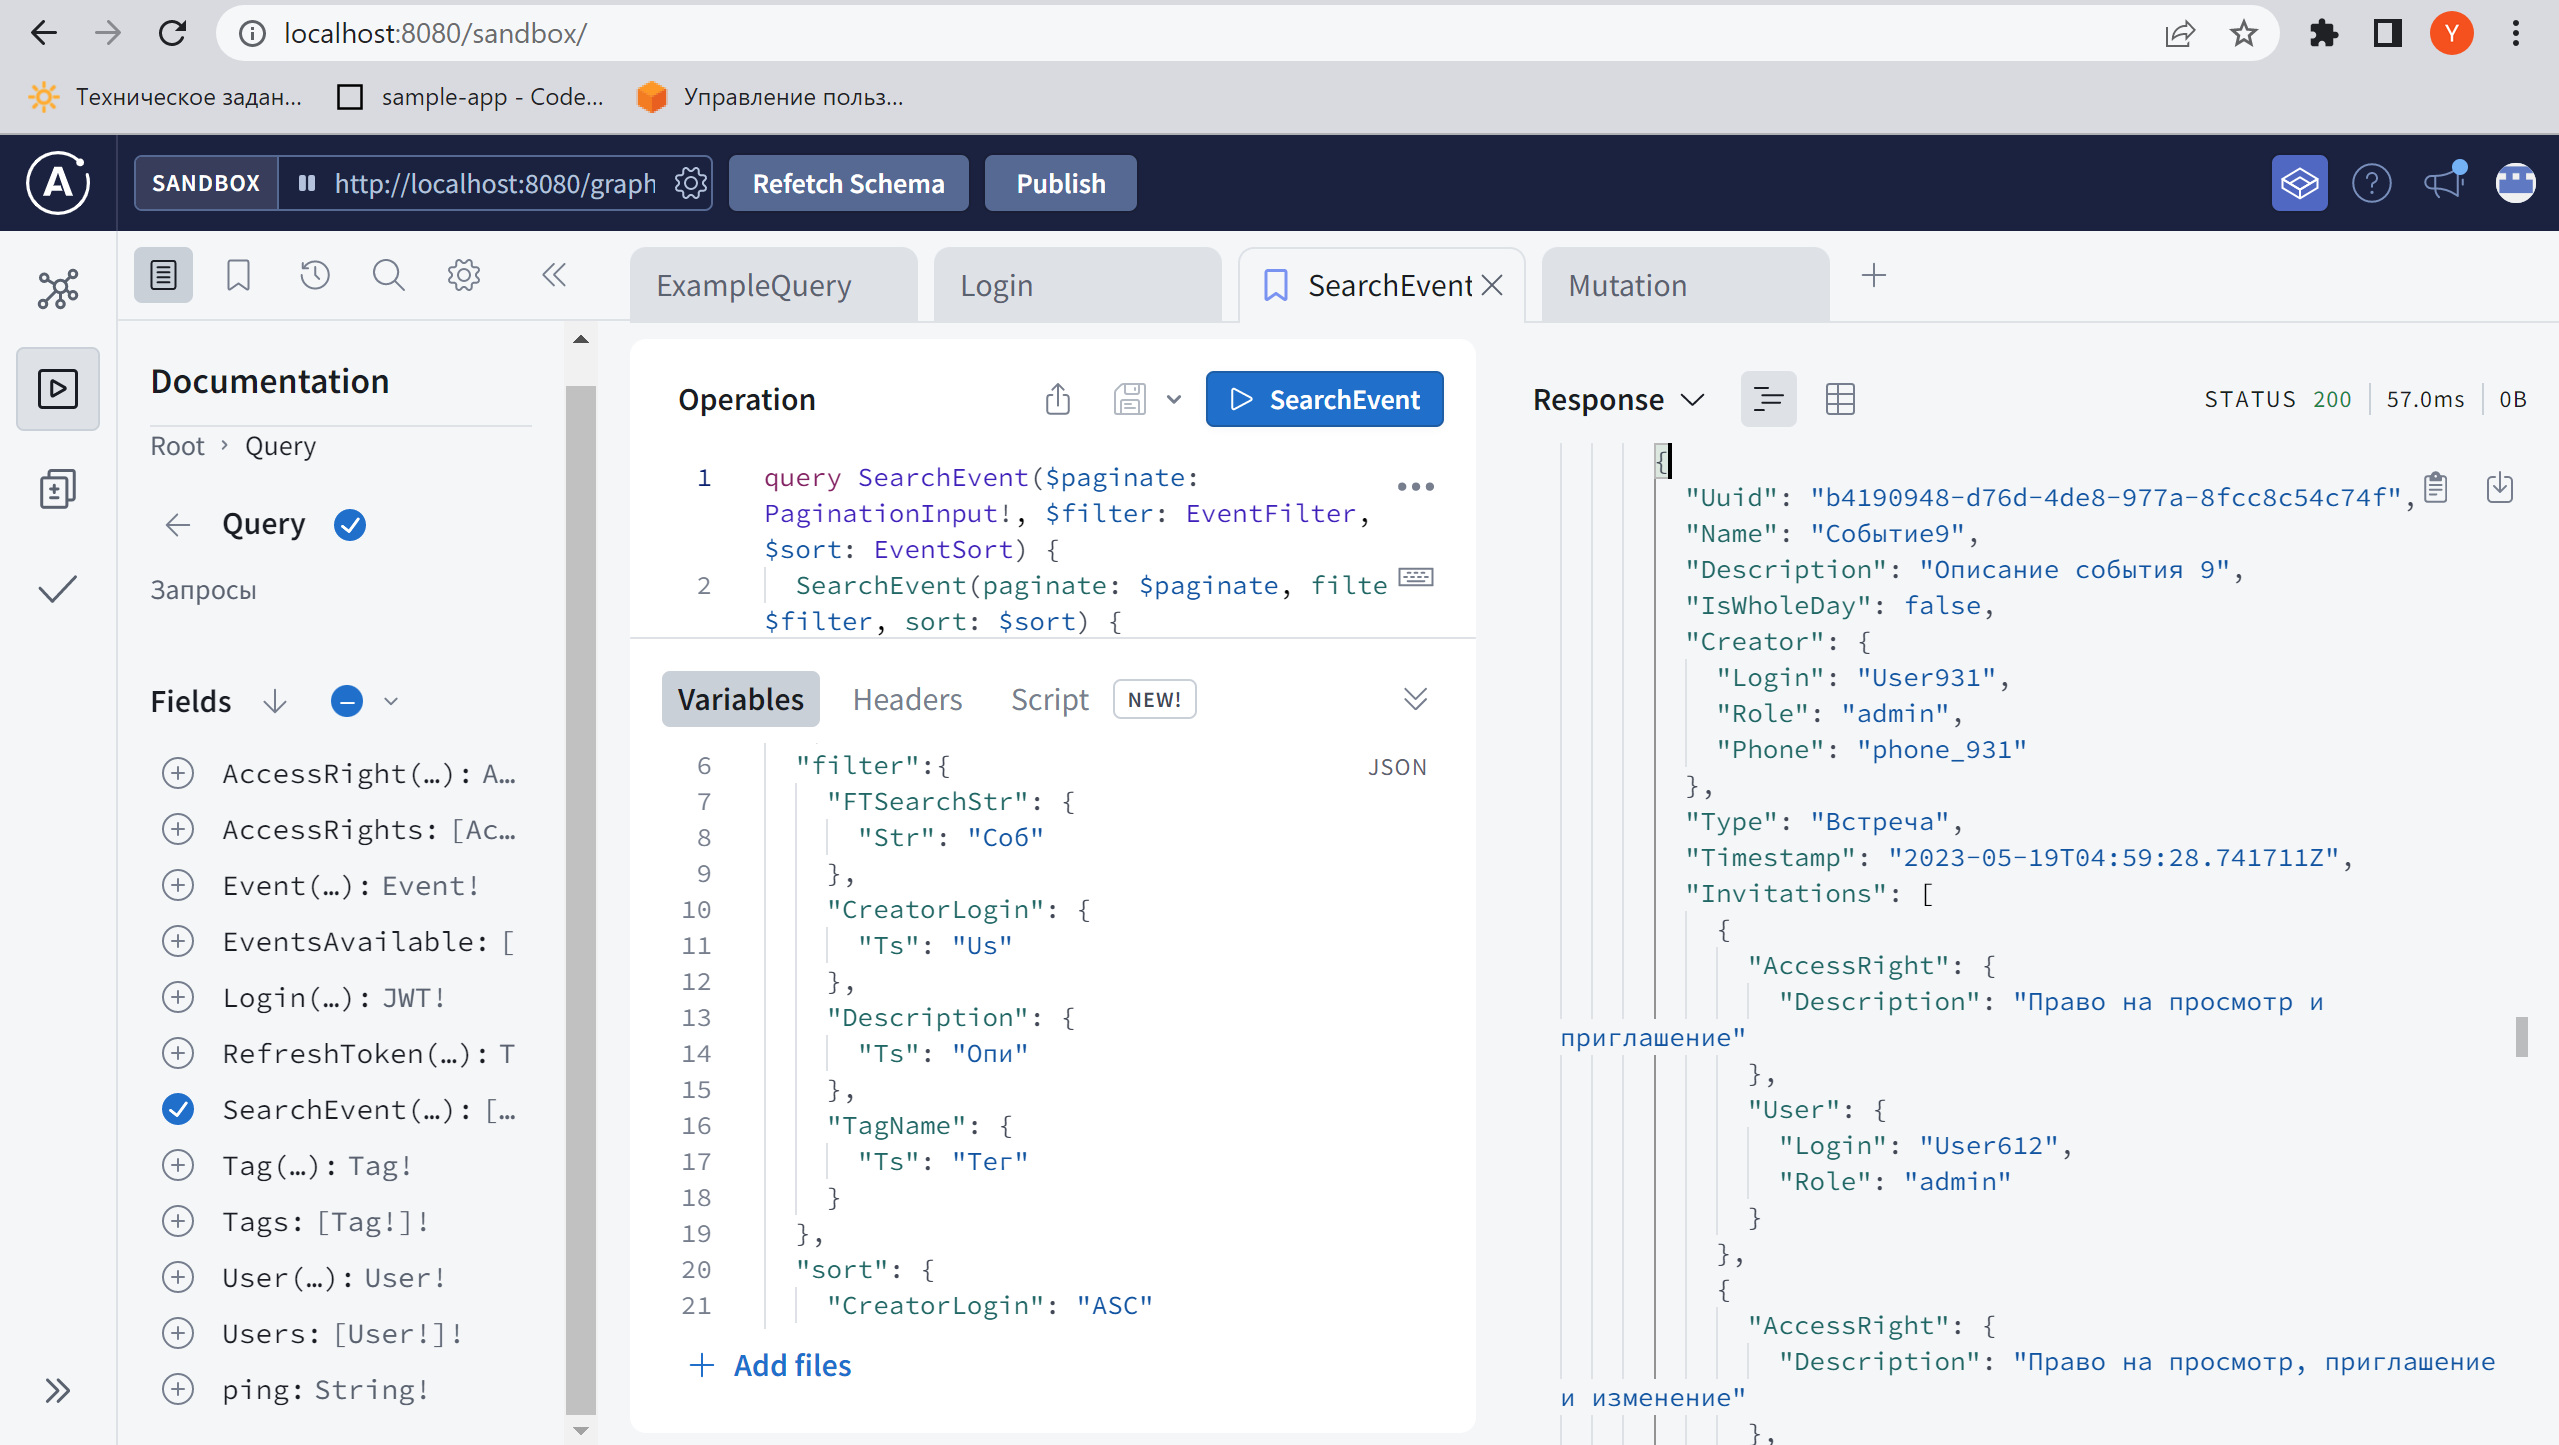
\includegraphics[width=1\linewidth]{assets/images/SearchEvents.png}
	\caption{Поиск событий с фильтрами и сортировкой}
	\label{fig:search-events}
\end{figure}

\begin{figure}[ht!]
	\centering
	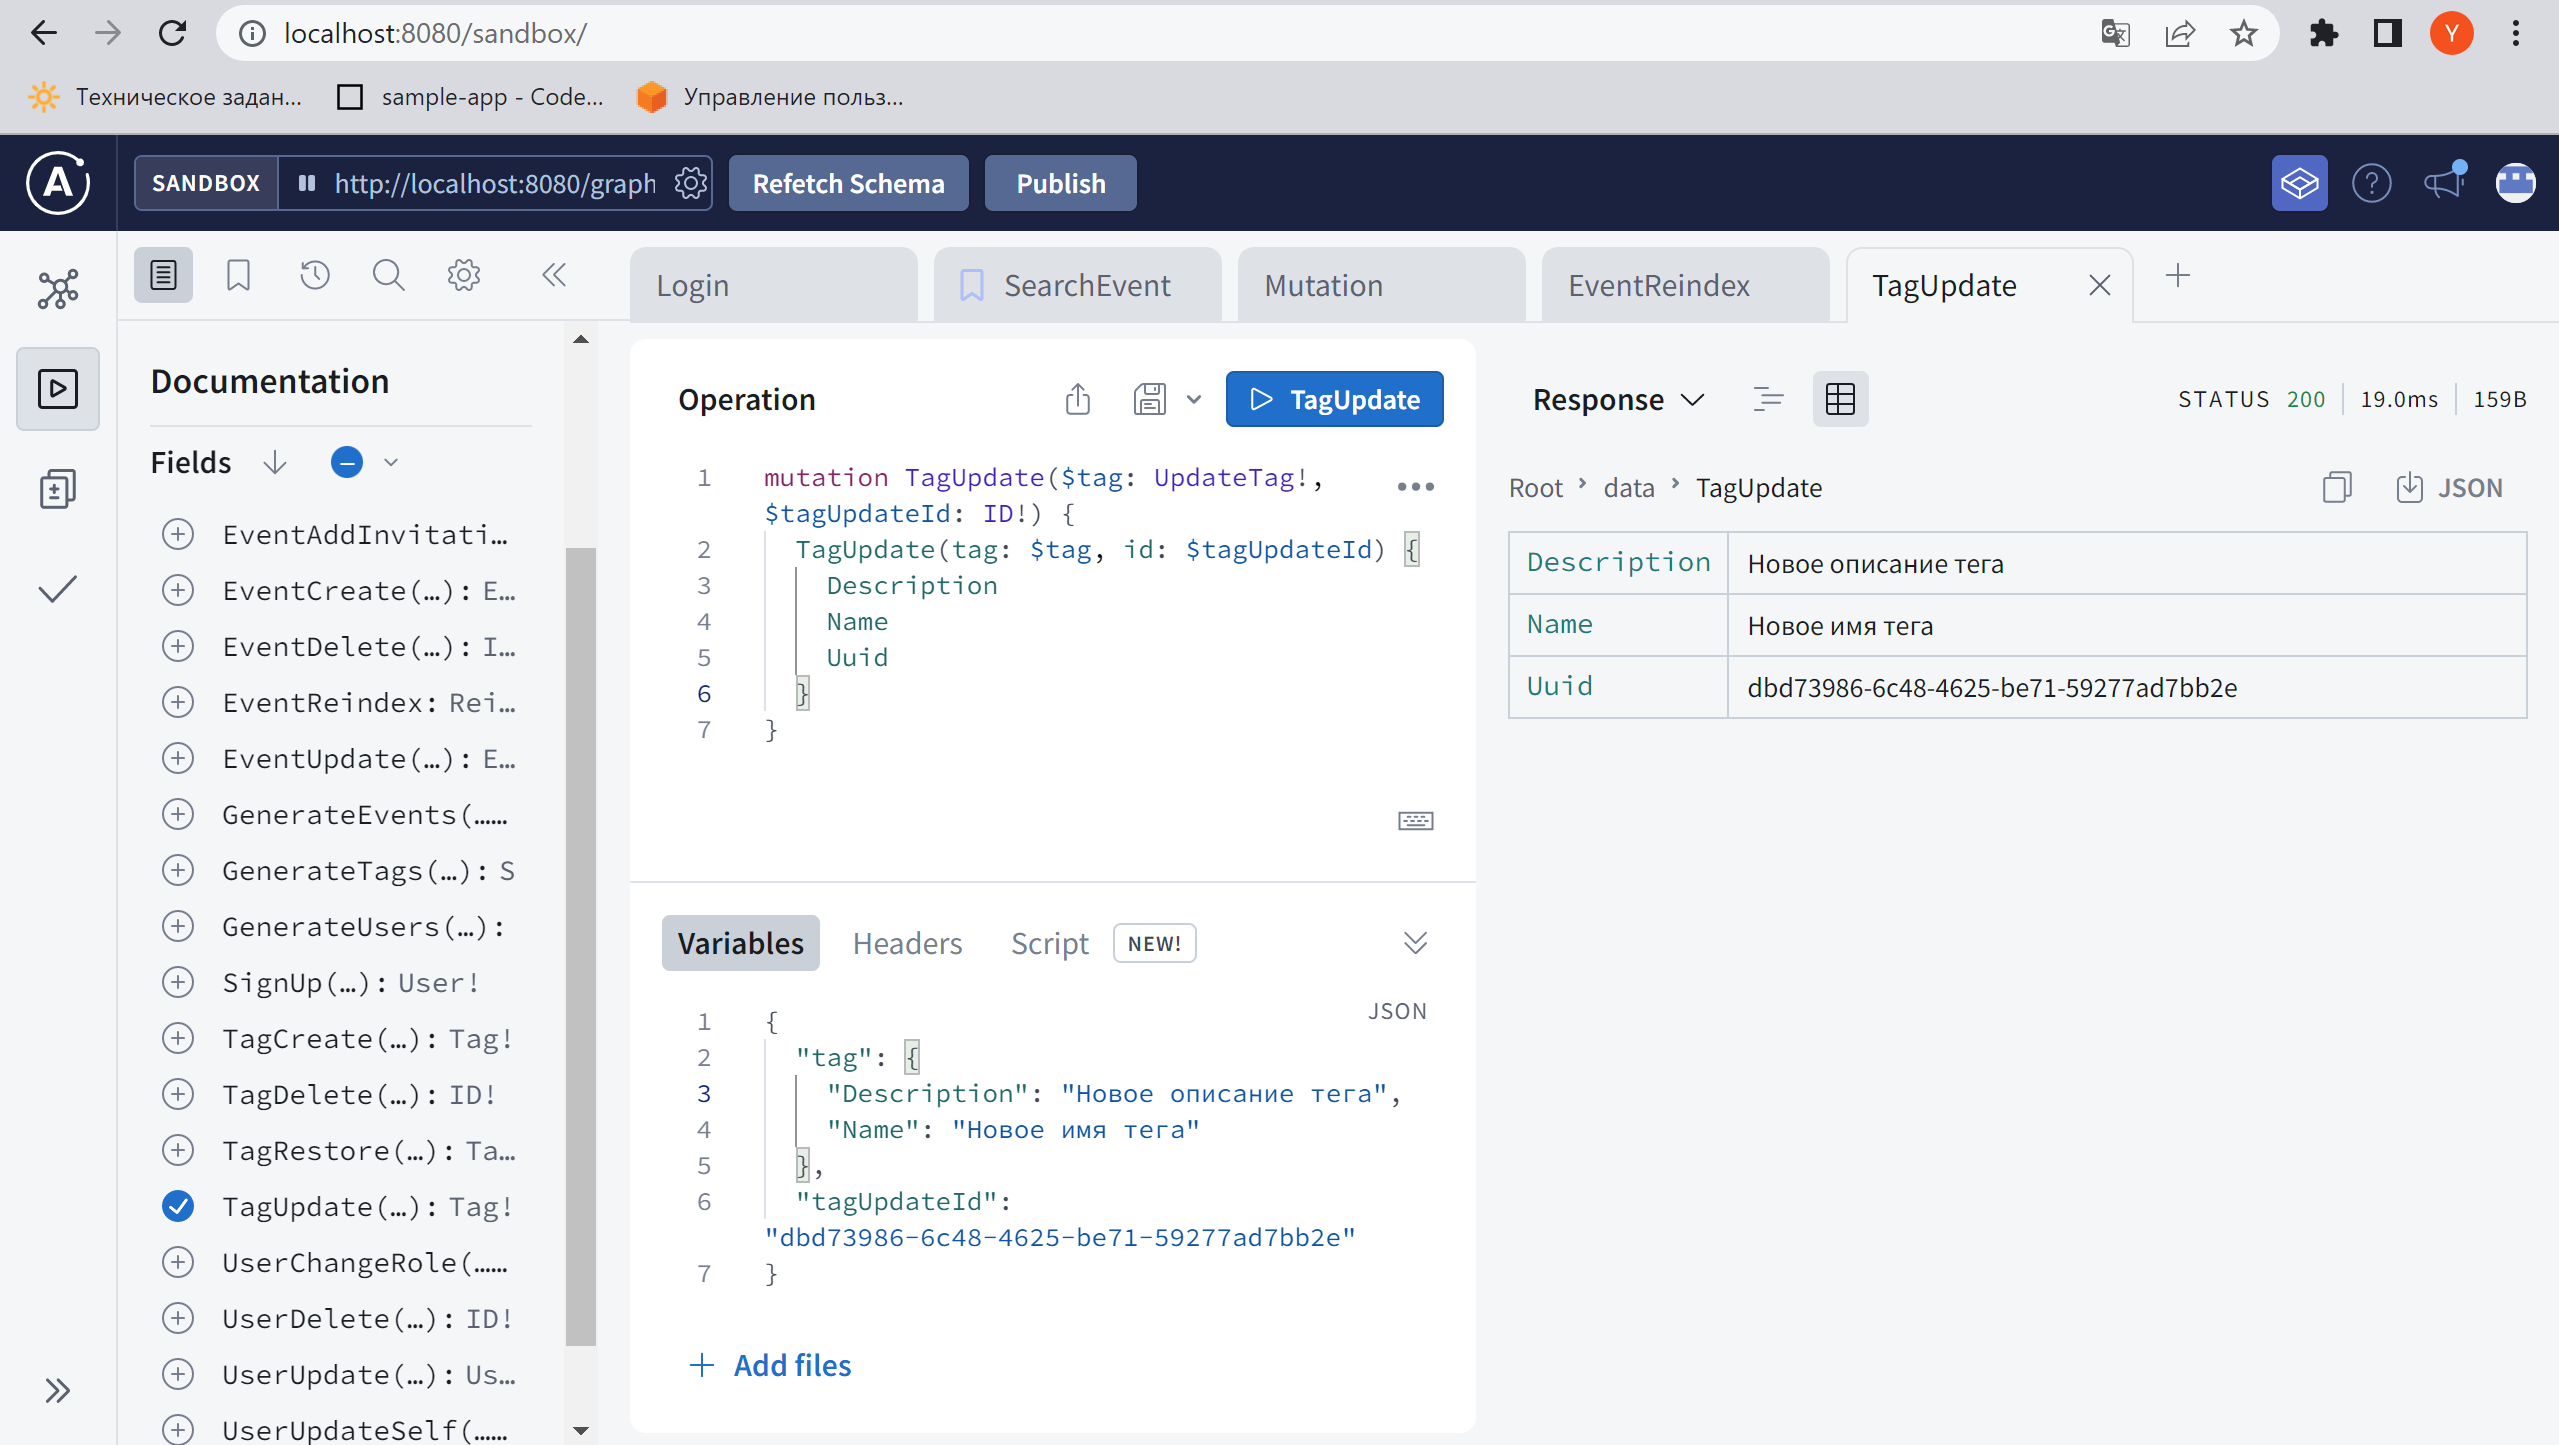
\includegraphics[width=1\linewidth]{assets/images/Tags.png}
	\caption{Обновление тега}
	\label{fig:tag}
\end{figure}

\begin{figure}[ht!]
	\centering
	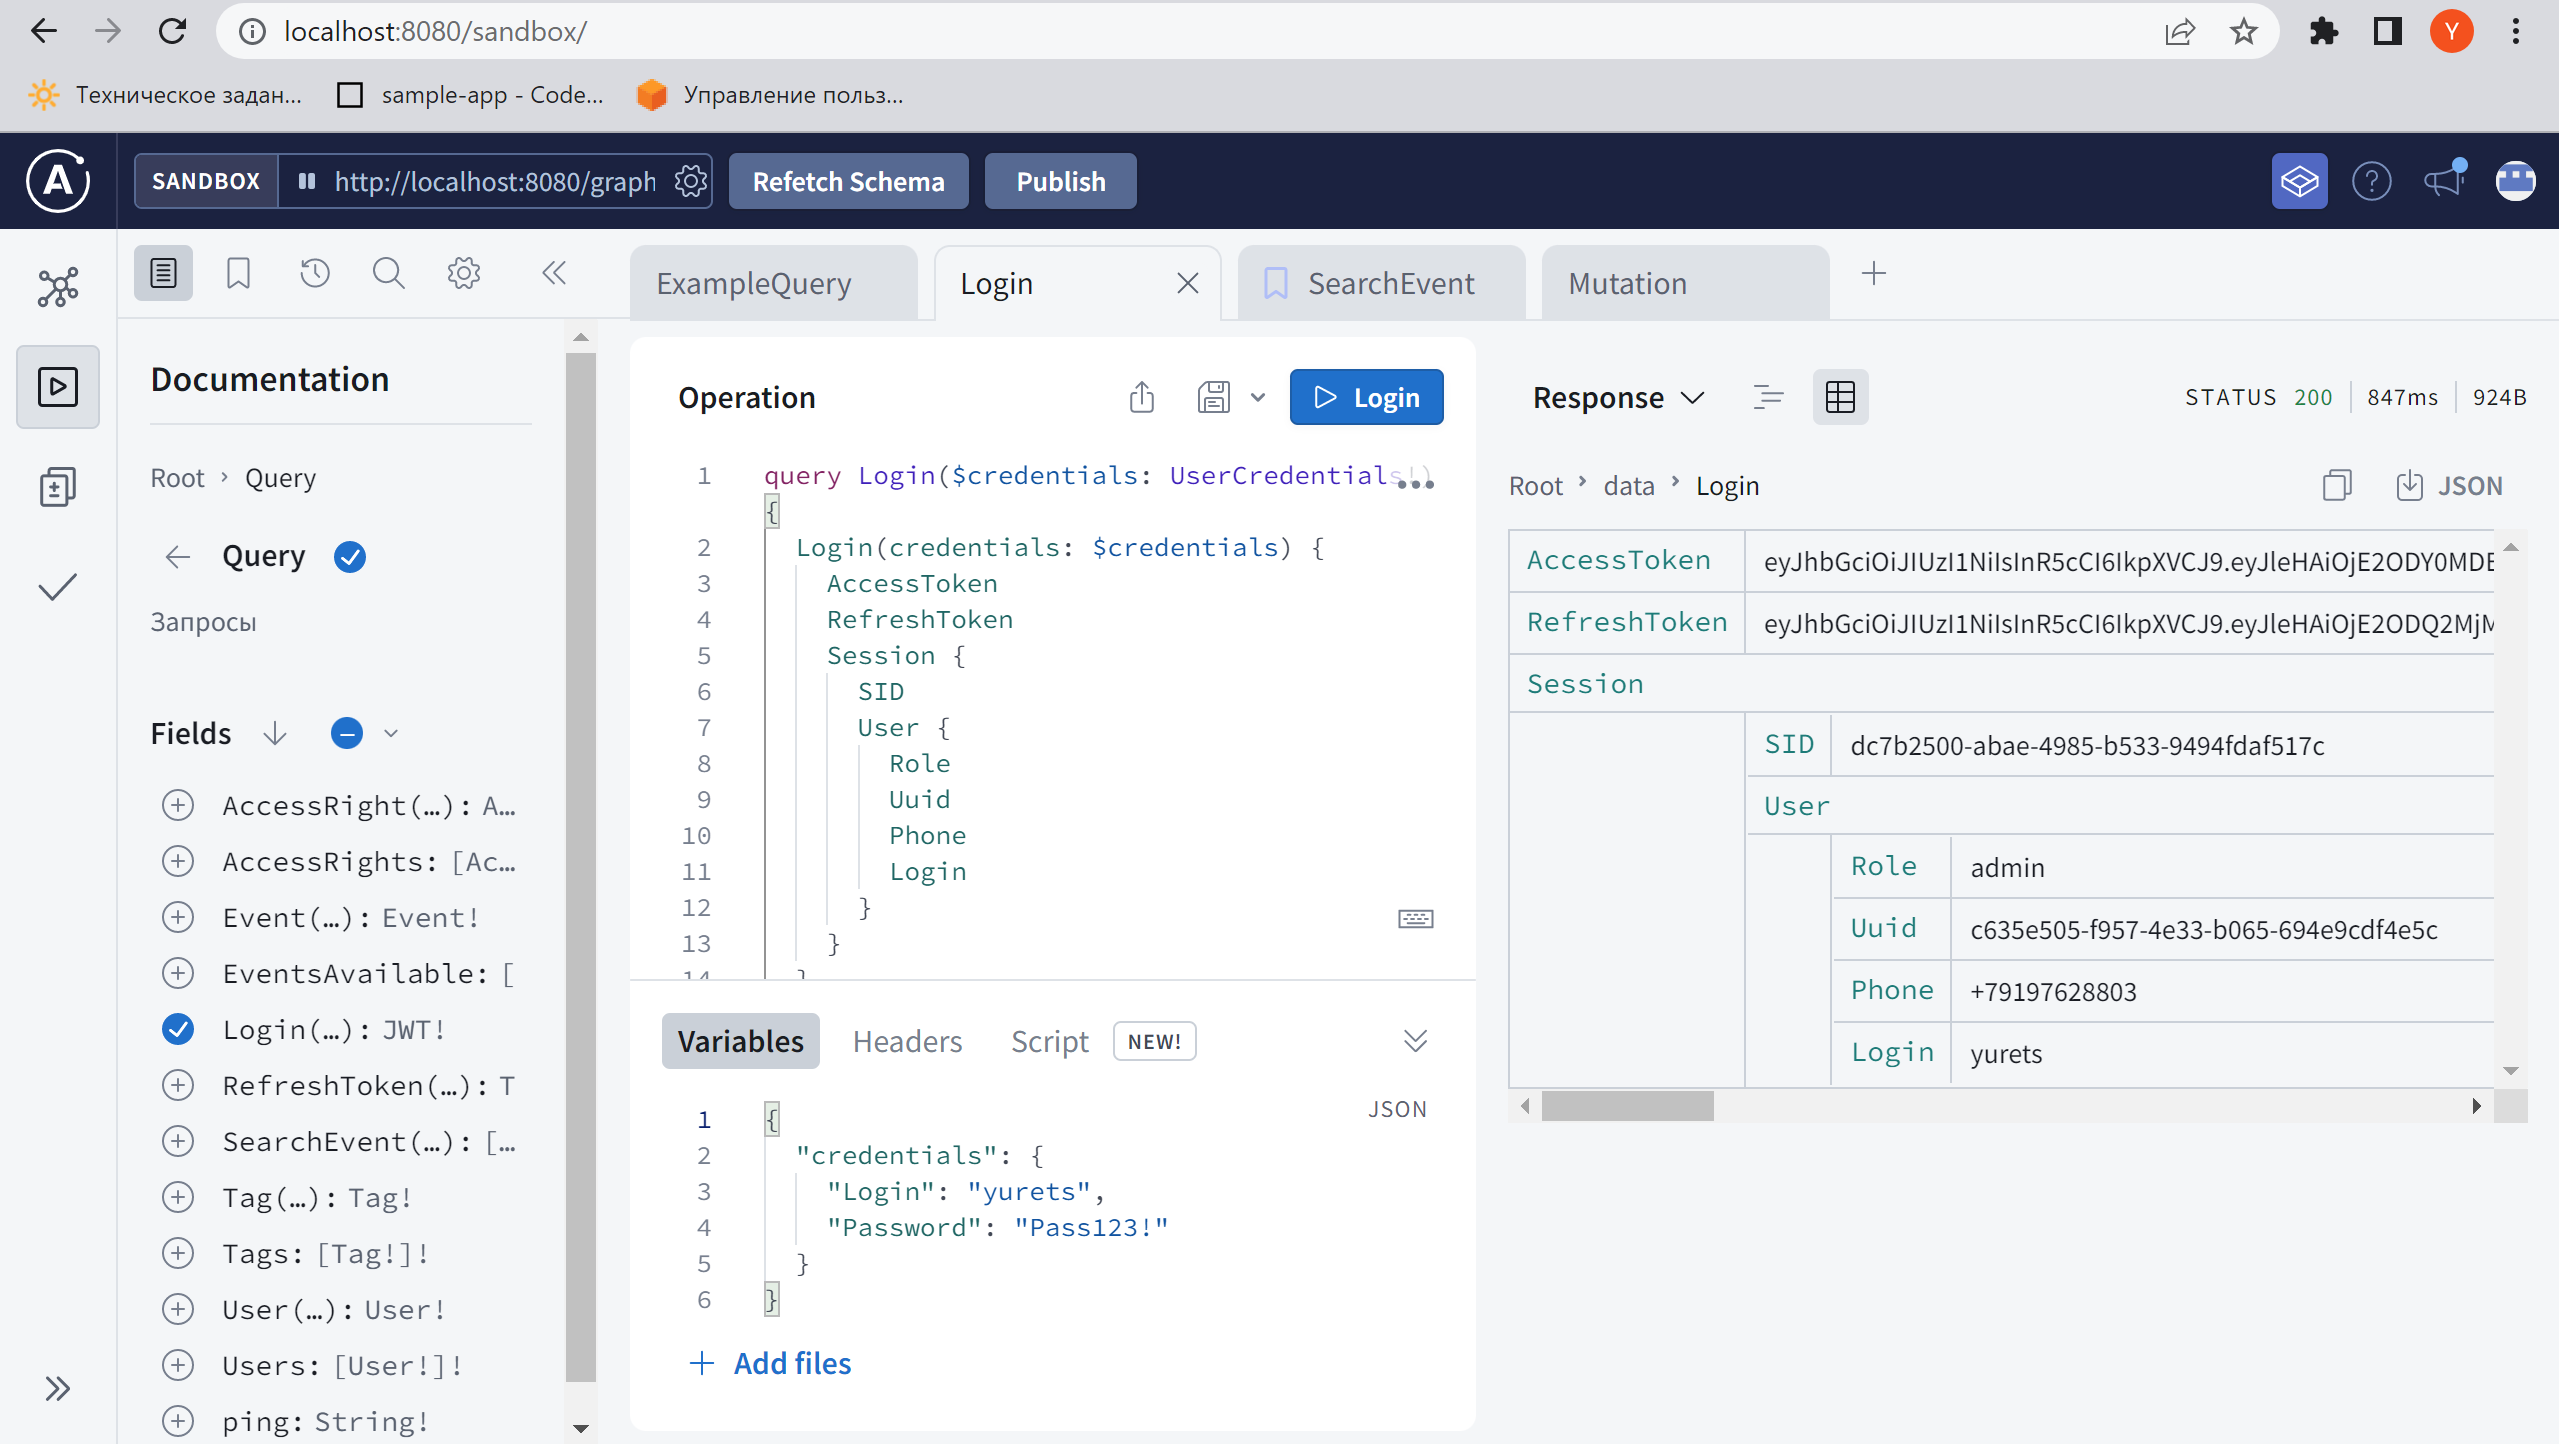
\includegraphics[width=1\linewidth]{assets/images/Login.png}
	\caption{Вход в систему (получение токена)}
	\label{fig:login}
\end{figure}


